\chapter{Results}\label{c:results}
In the following chapter we present the results from implementing the in \cref{c:method} introduced methods in the same order. We start by giving an interpretation of the networks behaviour in simulation with a subsequent parameter study.\\
Afterwards, the control approach is discussed and both derivations are briefly compared. To that important implementation details are explained to facilitate acceptable performance. It is also illustrated that the network as described acts more as an open loop controller. Control is displayed with both a dynamic system as well as a network as the underlying system to control.\\
As a next step, the results on the learning are presented and a parameters study is conducted for selected parameters and corresponding values. Also different sequences for learning are considered.\\
Lastly all of the previous steps are combined in an attempt to control a system.

\section{Results on the Simulation from \cref{sec:simulation}}\label{sec:res_simulation}
\subsection{Toy Example}
\begin{figure}[h!]
	\centering
	\centering
	\includegraphics[width=\textwidth]{../../plots/Simulation/basic_example.pdf}
	\caption{Baseline example}
	\label{fig:sim_res_1}
\end{figure}

The results from simulating the network with given input $\bmu{c}(t)$ can be seen in \cref{fig:sim_res_1}. In this scalar example the ODE
\begin{equation}\label{eq:leaky_integration_example}
\dot{x} = -10x +c(t)
\end{equation}
is simulated with 2 neurons. One neuron corrects the network simulation of the system up and down respectively. As shown before this correction happens immediately after each spike by adding weights of the relevant decoding vector to the trajectory. Since this example is following a scalar variable with 2 neurons the decoding matrix $\bmu{\Gamma}\in \mathbb{R}^{1\times2}$ and set to $\left[0.09,-0.09\right]$ for this example. This can be seen in \cref{fig:sim_res_1}, the neural network simulation jumps up after each spike by 0.09 is added. The external input follows a linear increase until 0.15s after which it remains constant.\\
For reference a conventional numeric solution is given which lies directly between the two neurons threshold, visualized with dotted lines.\\
\begin{figure}[h!]
	\centering
	\begin{subfigure}[t]{0.49\textwidth}
		\centering
		\includegraphics[width=\textwidth]{../../plots/Simulation/small_lambdaD.pdf}
		\caption{Reduced Readout Decay rate}
		\label{fig:sim_low_lambda}
	\end{subfigure}
	\hfill
	\begin{subfigure}[t]{0.49\textwidth}
		\centering
		\includegraphics[width=\textwidth]{../../plots/Simulation/small_gamma.pdf}
		\caption{Reduced Threshold}
		\label{fig:sim_low_gamma}
	\end{subfigure}
	\caption{Variation of Readout Decay and Decoder for simple 1D system.}
	\label{fig:sim_res_2}
\end{figure}
Already for this toy example different parameters can be tuned to get different results. In \cref{fig:sim_low_lambda} the readout decay is reduced compared to \cref{fig:sim_res_1} which reduces how fast the output tends to zero. This also elevates the importance of a single spike as it has longer lasting effects on the output, seen by the system showing fewer spikes than before.\\
Alternatively, if the decoding weights can be scaled to let each spike make a smaller change in the output seen in \cref{fig:sim_low_gamma}. Since the threshold is closely tied to the Decoding weights this also reduces the spike threshold and therefore yields more accurate results.\\

\subsection{Toy example in 2D}

\begin{figure}[h!]
	\centering
	\includegraphics[width = \textwidth]{../../plots/Simulation/simple_2d.pdf}
	\caption{Simple 2D example with numerical solution and spike response. Curves for $x$ in yellow/blue. Curves for $y$ in purple/red. The networks output closely tracks the perfect numerical solution. For the network each decoding vector was chosen from a normal distribution and normalized to $\left\lVert\bmu{\Gamma}_i\right\rVert_2 =0.3$. Beneath a raster plot for each spiking neuron. On the left the threshold for each neuron's projected error.}
	\label{fig:sim_res_simple}
\end{figure}

In two dimensions the network also allows for a geometric interpretation. For this we let the network simulate a simple leaky integration of inputs as in \cref{eq:leaky_integration_example} but in two dimensions. In \cref{fig:sim_res_simple} we can see that at different times different neurons are activated. The corresponding fires according to the phase plot on the right in \cref{fig:sim_res_simple}.\\
In detail this can be seen in \cref{fig:sim_res_geometric}. Here a simulation is run with just 4 neurons, covering the two axis. The lines in the bottom right panel show the thresholds of each neuron in the direction of its projected error. As the input $\bmu{c}$ is fed into the net, the error rises while the network remains dormant. This can be seen in the zoom-in section of \cref{fig:sim_res_geometric} in the bottom left. This error is also shown as an orange arrow of originating from the origin in the bottom right panel. The Voltage, and thus the error, rise until the threshold is reached. After a spike is fired, indicated by the spike plot underneath on the left and the crossing of threshold in dark blue, the network output is shifted by adding $\bmu{\Gamma}_i$ to it. This can also be observed, as the error in the bottom left panel moves closer to the origin. With the continuous input $\bmu{c}$ next the threshold of the neuron in green is reached, causing a spike to be fired resetting the error again and adding a jump in negative $y$ direction to the network output. The spike moves the error orthogonal to the threshold line closer to the origin. In networks with more neurons this jump can reduce or increase the errors of other neurons. In the perspective of the neuron with turquoise limit, a spike of the dark blue neuron directly increases its perceived error. If no regularization in terms of $\mu$ or $\nu$ is used, a spike from one side of the threshold would move the signal exactly to the opposite neuron threshold.
\subsection{Geometric Interpretation in 2D}
\begin{figure}[h!]
	\centering
	\includegraphics[width = \textwidth]{../../plots/Simulation/2d_simple_spikes.pdf}
	\caption{Simple 2D example with numerical solution and spike response. Curves for $x$ in yellow/blue. Curves for $y$ in purple/red. The networks output closely tracks the perfect numerical solution. For the network each decoding vector was chosen from a normal distribution and normalized to $\left\lVert\bmu{\Gamma}_i\right\rVert_2 =0.3$. Beneath a raster plot for each spiking neuron \\ On the left the threshold for each neuron's projected error. The quadratic cost $\mu$ = 0.3.}
	\label{fig:sim_res_geometric}
\end{figure}


\subsection{Importance of Feedforward weights}
So far we have not given much attention to Feedforward weights. Yet they play a crucial rule in the performance of our network as seen in \cref{fig:sim_res_3}. Here we simulate again a simple leaky integration as in \cref{eq:leaky_integration_example} however this time in 2D. With the output, in each test we also plot the bounding box of neuron thresholds for the projected error.\\
The bounding box of the error is the normal to each of the decoding weights. In \cref{eq:x_hat} the network output gets the $i$th column $\bmu{\Gamma}$ added when the $i$th neuron spikes. From the minimization of the cost we know that the spike of neuron $i$ reduces the error in projected by $\bmu{\Gamma}_i$. If we know imagine the origin of the \cref{fig:sim_res_3} l to always be on top of the true trajectory of $\left[x ,\ y\right]^T$, the network's error is just deviation from the origin.\\
As can be seen in the \cref{fig:sim_res_3}, the more uniform the decoding weights are distributed, the better the network accuracy. In \cref{fig:sim_perfect_gamma}, it is possible to see the spiking neurons engage after another as the input is alternating. This can also be observed in \cref{fig:sim_random_gamma} although higher irregularity in the spiking can be observed compared to \cref{fig:sim_perfect_gamma}. This is because in the second quadrant of the projected error plot more neurons are more densely packed. Meanwhile in the third and the fourth quadrant approximately 3 neurons cover the bottom limit (if their lines are extended). This cone comprised of the dark blue and yellow neuron engage in rapid alternating firing in order to keep follow the trajectory.\\
In the last example a particular bad choice of Feedforward weights is displayed. Here, the box is not fully enclosed by neurons, resulting in the network to be completely blind to errors in these directions.
\begin{figure}[h!]
		\centering
	\begin{subfigure}[t]{0.6\textwidth}
		\centering
		\includegraphics[width=\textwidth]{../../plots/Simulation/2d_perfect_gamma.pdf}
		\caption{Network }
		\label{fig:sim_perfect_gamma}
	\end{subfigure}
	\hfill
	\begin{subfigure}[t]{0.6\textwidth}
		\centering
		\includegraphics[width=\textwidth]{../../plots/Simulation/2d_random_gamma.pdf}
		\caption{Reduced Threshold}
		\label{fig:sim_random_gamma}
	\end{subfigure}
	\hfill
\begin{subfigure}[t]{0.6\textwidth}
	\centering
	\includegraphics[width=\textwidth]{../../plots/Simulation/2d_bad_gamma.pdf}
	\caption{Reduced Threshold}
	\label{fig:sim_bad_gamma}
\end{subfigure}
	\caption{Network output after leaky integration of oscillating input with different decoding vectors.}
	\label{fig:sim_res_3}
\end{figure}


\subsection{Bigger Systems}
\begin{figure}[h!]
	\centering
		\includegraphics[width=\textwidth]{../../plots/Simulation/big_system.pdf}
	\caption{Trajectory of dynamic mass spring system with 100 masses and 2 thousand neurons. Only the first 3 trajectories are plotted and the spikes for the first 200 neurons.	}
	\label{fig:big_systems}
\end{figure}

So far we have only looked simple systems in 1D or 2D. However our network can also simulate more complex higher dimensional systems.
In the example in \cref{fig:big_systems} we simulated a linear n-mass spring system with the dynamics
\begin{equation}
	m_i\ddot{x}_i = K\cdot \begin{bmatrix}
	1&-2&1
	\end{bmatrix} \cdot	\begin{bmatrix}
	x_{i-1}\\
	x_i\\
	x_{i+1}
	\end{bmatrix} + c_i(t).
\end{equation}
The external forces were each offset sinusoidal waves with varying frequency and amplitude for the first 3 masses and random forces for the rest. As can be seen from the figure, the network perfectly overlays the numerical solution.


\subsection{Varying cost parameters $\mu,\nu$}
\begin{figure}[h!]
	\centering
	\begin{subfigure}[t]{0.6\textwidth}
		\centering
		\includegraphics[width=\textwidth]{../../plots/Simulation/2d_cost_none.pdf}
		\caption{Network }
		\label{fig:sim_no_cost}
	\end{subfigure}
	\hfill
	\begin{subfigure}[t]{0.6\textwidth}
		\centering
		\includegraphics[width=\textwidth]{../../plots/Simulation/2d_cost_nu.pdf}
		\caption{Reduced Threshold}
		\label{fig:sim_nu_cost}
	\end{subfigure}
	\hfill
	\begin{subfigure}[t]{0.6\textwidth}
		\centering
		\includegraphics[width=\textwidth]{../../plots/Simulation/2d_cost_mu.pdf}
		\caption{Reduced Threshold}
		\label{fig:sim_mu_cost}
	\end{subfigure}
	\caption{Network output after leaky integration of oscillating input with different decoding vectors.}
	\label{fig:sim_res_4}
\end{figure}

\section{Results on the control}\label{sec:res_control}
For the evaluation of the results for the control problem derived in \cref{sec:control} we first note a few important implementational details in order to get useful results. \\
Afterwards we compare the performance of the two different derivations from \cref{ssec:control_dynamics,ssec:extension} and briefly discuss the necessary condition for the control schemes to function.
Lastly we take a closer look at the main reason for the control to work and how we can adopt it to our learning problem in \cref{sec:learning}.
With the chosen network architecture, robustness against neuron failure and noise has already been tested and verified. To avoid repetition, specific testing into these topics is waived.
\subsection{Acceptable error}
Due to the networks discrete nature of spikes, any error below the threshold cannot be eliminated. This threshold is fixed by the fact that a spike of neuron $i$ produces a constant change in the signal given by the decoding $\bmu{\Gamma}_i$. Accuracy levels commonly observed with classic control schemes and numerical methods are unattainable due to this restriction. On the other hand, error is also bound from above by the threshold. While it is theoretically possible to achieve arbitrarily small errors by scaling $\bmu{\Gamma}_i$, the error is bound by the spiking threshold  $\frac{\|\bmu{\Gamma}_i\| + \mu}{2}$ and the only considered in the directions projected by $\bmu{\Gamma}$.


\subsection{Implementation details}
Before any simulation can be run it is important that certain detail in the implementation are set in the correct order for the results to make sense.

\subsubsection{Multiple spikes per timestep}
Although this also applies for the simulation step in \cref{sec:res_simulation}, its affects are much more pronounced in the control setting.\\
\paragraph{Single Spike}
As the dynamics outlined suggest the simulation step includes a check if a threshold has been reached. \\
A simple implementation in MatLab pseudo code is seen in \cref{lst:single_spike}.

\begin{lstlisting}[language=Matlab, caption=Single spike implementation,label=lst:single_spike]

for t_step = 1:N_step
	V = update_Voltages(V,dt,Ws,Wf,c,...);
	[value, index] = max(V-Threshold);
	spikes(index,t_step) = 1;
	V = V + Wf(:,k);
	...
end
\end{lstlisting}
While this works for a variety of problems it does not give results for any given system and reference trajectory.\\
Especially problems with an abrupt change underperform since the network is only allowed to correct the error by one spike. However by jumps and rapid changes this is not sufficient to compensate errors and then networks struggles for many iterations to recover, ruining the overall accuracy in the process.
\paragraph{Parallel Spikes}
Now the direct way to fix this to find all neurons that have reached their thresholds. Since networks have many neurons, letting every neuron spike increases the networks ability to correct errors. A potential implementation is seen in \cref{lst:multi_spike}.
\begin{lstlisting}[language=Matlab, caption=Letting every neuron spike in parallel,label=lst:multi_spike]

for t_step = 1:N_step
	V = update_Voltages(V,dt,Ws,Wf,c,...);
	spiking_neurons = V>Threshold; % procudes a list
	spikes(spiking_neurons,t_step) = 1;
	V = V + Wf(:,spiking_neurons);
	...
end
\end{lstlisting}
The problem with this implementation is that the error gets tracked by multiple neurons simultaneously and also in both in positive and negative direction. To illustrate this we consider a simple example where we have a single control variable $u$ and $2N$ neurons, where $N$ neurons track positive and negative error respectively.\\
Disregarding noise, the threshold is reached by $N$ neurons synchronously. As long as the total error is larger than the compensation of $N$ neurons in the first place, this works just fine. However this is not permanent and at some point all $N$ neurons firing overly depolarize the opposite side neurons to the extend that they all fire in the next iteration regardless of the real system error.\\
The root cause is that a single spike influences the whole network. In this extreme case 1 spike resets all other $N-1$ neurons that were spiking as well and therefore would not give any performance boost compared to the previous approach.\\
The network with this implementation behaves normally while a rapid change is present but will evolve into $N$ neurons spiking in alternating cadence respectively.\\
To remedy this it is necessary that one dimension of the error is only projected onto two neurons. While this can be achieved by carefully selecting the decoder it is not a generic approach. Moreover this reverses the idea of multiple neurons tracking the error for robustness.\\
Therefore we need to let a single neuron spike multiple times.

\paragraph{Multiple Spikes}\label{p:multiple_spikes}
The correct way to handle this problem is to allow more than one spike per time step but compute each spike's change in the network separately. This way we can achieve the necessary performance without the problems of the previous approach. A implementation of such a regime is seen in \cref{lst:correct_spike}

\begin{lstlisting}[language=Matlab, caption=Letting each neurons spike as many times a necessary while computing each spike's influence sequentially.,label=lst:correct_spike]

for t_step = 1:N_step
	V = update_Voltages(V,dt,Ws,Wf,c,...);
	[value, index] = max(V-Threshold);
	while value > 0
		spikes(index,t_step) = 1;
		V = V + Wf(:,k);
		...
		[value, index] = max(V-Threshold);
	end
end
\end{lstlisting}
In order to retain biologic plausibility, it is necessary to limit the number of spikes fired in one time step. While this is not a problem in most cases when hyper-parameters are properly tuned, it can be an issue if there are sudden jumps or rapid transitions.\\

\subsubsection{Slow Connectivity Term}
In their derivation consider network in the limit for $N\rightarrow \infty$ neurons. Specifically the derivation arrives at
\begin{equation}
\begin{aligned}
\dot{\bmu{V}}(t)= & \bmu{\Omega}^T \bmu{B}^T\left(\dot{\hat{\bmu{x}}}(t)-\dot{\bmu{x}}(t)\right)-\mu \lambda_d \dot{\bmu{r}}(t) \\
= & \bmu{\Omega}^T \bmu{B}^T \bmu{A} \bmu{L} \bmu{V}(t) \\
& +\left(\mu \lambda_d \bmu{\Omega}^T \bmu{B}^T \bmu{A} \bmu{L}+\mu \lambda_d^2 \bmu{I}-\frac{1}{\lambda_d} \bmu{\Omega}^T \bmu{B}^T \bmu{B} \bmu{\Gamma}\right) \bmu{r}(t) \\
& -\left(\bmu{\Omega}^T \bmu{B}^T \bmu{B} \bmu{\Omega}+\mu \lambda_d^2 \bmu{I}\right) \bmu{o}(t) \\
& +\bmu{\Omega}^T \bmu{B}^T(-\bmu{A} \hat{\bmu{x}}(t)+\dot{\hat{\bmu{x}}}(t))
\end{aligned}
\end{equation}
where $$\bmu{L} = \left(\bmu{B\Omega\Omega}^T\bmu{B}^T\right)^{−1}\bmu{B\Omega}$$ is the pseudo-inverse of $\left(\bmu{B\Omega}\right)^T$. Our focus is now set on the terms in front of the rate. As \cite{huang_optimizing_2017} and the original derivation in \cite{boerlin_predictive_2013} argue the term $\mu\lambda_d^2$ vanishes in the limit and can therefore be neglected, yielding the above result for $\bmu{W}^s$ above in \cref{eq:Ws_wrong}.\\
However in the testing it was noticed that this derivation only produces acceptable results for a small range of values for $\lambda_d$, explicitly $\lambda_d \leq 20$. For values above the performance deteriorates rapidly if not a large number of neurons is considered.\\
After testing the relative importance of terms it was noted that the term $\mu\lambda_d^2$ does improve the performance with a smaller number of neurons significantly compared to the other terms and was therefore added in the results following below.\\
Furthermore the authors' examples clearly indicate their use of the extra term as well in the calculation of $\bmu{W}^s$. This, in addition to our testing, confirms the permanent addition of $\mu\lambda_d^2$.

\subsection{Network as the controller}
Now we start to compare both methods against each other. Except of an introductory example we will mostly outline observed differences.
Both methods require to receive the desired state trajectory as input. To test their usability, different size problems as well as configurations of $\bmu{B}$ and $\bmu{C}$ will be tested.\\
For testing purposes, we set the test system $\bmu{A}$ to
\begin{equation}
	\bmu{A} = \begin{bmatrix}0 & 1\\-1 & 10\\\end{bmatrix}.
\end{equation}
Additionally, for the $N=50$ neurons we choose their instantaneous decoding weights $\bmu{\Omega}$ randomly and normalize them to 0.01 without any rate decoding $\bmu{\Gamma}$.

\subsubsection{\ac{SISO} systems}
Both methods performed identically well with \ac{SISO} systems. Error levels are limited by the scaling of $\bmu{\Gamma}$ with single spike deviations from the target.\\
To influence the control behaviour, different parameters can be tuned. Increasing costs $\mu$ and $\nu$ will lead to a increased settling time. Increasing the number of neurons or the number of allowed spikes per neuron will improve the error, especially the immediate increase seen in the top panel of \cref{fig:step_compare}. Lastly, the scale of the rate encoding $\bmu{\Gamma}$ can be tuned to lower the rise time. However this can lead to overshoot, seen in the bottom panel of \cref{fig:step_compare}. In general the rate encoding $\bmu{\Gamma}$ introduced with the control is mainly responsible to reduce the amount of spiking in the network. As can be seen in \cref{fig:step_compare} the absence of $\bmu{\Gamma}$ is only noticeable in the slower settling time. With purely instantaneous encoding the control signal has to be constructed for each time-step from zero only with spikes. This extensive firing causes quadratic costs $\mu\|\bmu{r}\|^2_2$ to rise and slow down spiking of repeatedly firing neurons. Thanks to a large number of neurons for this problem and low quadratic costs $\mu = 1\cdot10^{-6}$ this is not a problem in the shown example. On the other side the addition of $\bmu{\Gamma}$ brings additional momentum, given by the slower changing rates $\bmu{r}$, that in case of sudden changes first needs to be counteracted, seen by the overshoot in \cref{fig:step_compare}.\\
In the presence of noise, the control scheme with the direct error performed slightly better. This was expected as the explicit error term in the voltage equation benefits the compensation of noise in the network.
\begin{figure}
	\centering
	\includegraphics[width=\textwidth]{../../plots/Control/compare_step_both_methods.pdf}
	\caption{Step response for simple 2D system and. Both runs are identical except of $\bmu{\Gamma} = 0$(top) and $\bmu{\Gamma} = 100\cdot\bmu{\Omega}$. Both approaches performed identically.}
	\label{fig:step_compare}
\end{figure}



\subsubsection{Suboptimal $\bmu{B}$, $\bmu{C}$ and \ac{MIMO}}
Difficulties arise when more complex problems are considered.\\
In order for the control schemes to work the necessary condition $\bmu{B}^T\bmu{C}^T \neq 0$ has to hold\cite{huang_dynamics_2019}. However the condition has to be understood as $\rank\left(\bmu{B}^T\bmu{C}^T\right) = \rank{\bmu{B}}$. Otherwise certain state variables cannot be controlled. These "invisible states" are neglected by the network. This limitation is shared between both methods. Reason behind that is
that the matrix $\bmu{B}^T\bmu{C}^T$ blinds the Voltage on projecting the error properly in \cref{eq:control_dyn_begin} and \cref{eq:direct_error_voltage}.\\
If $\bmu{B}^T\bmu{C}^T$ exhibits rank deficiency, certain neurons do not receive the input $\bmu{c}$. They are therefore only affected indirectly in \cref{eq:control_dyn_2} by the spiking of other neurons and not by the target trajectory. This results that either the output trajectory is not tracked in the first place or if the output is tracked, the internal states are moving freely.\\
To insure the rank condition this restricts the possibilities of $\bmu{B}$ and $\bmu{C}$.
If $\bmu{B} \in \mathbb{R}^{n\times J}$ and $\bmu{C} \in \mathbb{R}^{m\times n}$ we need to enforce that $m\geq J$. In order for $\bmu{B}^T\bmu{C}^T$ to have full rank $J$, it is necessary that $\bmu{C}^T$ has at least rank $J$ due to
\begin{equation}
	\rank\left(\bmu{B}^T\bmu{C}^T\right) \leq \min\left(\rank\left(\bmu{B}^T\right),\rank\left(\bmu{C}^T\right)\right) = \min\left(J,m\right)
\end{equation}

\subsubsection{Equivalence of $\bmu{\hat{x}}$ and $\bmu{x}$}
The derivation of error method to work it is crucial that the external input $\bmu{c}$ is accurately calculated from the reference by
\begin{equation}
	\dot{\hat{\bmu{x}}} = \bmu{A}\hat{\bmu{x}} + \bmu{c}.
\end{equation}
This represents an open loop controller without any feedback from the system itself. Even though the network output is directly part of the equation, the error term is present due to the definition of the voltage. In previous derivations this term was neglected after considering the limit of $N_{\text{neur}}\longrightarrow \infty$.\\
Now as both $\bmu{\hat{x}}$ and $\bmu{x}$ follow the same dynamics, it appears natural that they can be interchanged to allow for true feedback. When determining the network input $\bmu{c}$, using the actual network output present to compensate any errors. However in practice plugging this in \cref{eq:direct_error_voltage} can pose problems to the network, even if $\bmu{C}$ and $\bmu{B}$ are chosen ideally.\\
While they both follow the same dynamics, their values may be different. Yet even with tiny differences, $\bmu{c}$ can ruin the control completely.\\
After careful investigation, the problem stems from the aforementioned supposed equivalence for $\bmu{c}$.\\
To illustrate the problem we consider a 1D example.
\paragraph{$\hat{\bmu{x}} \neq \bmu{x}$}
The reason for control failure when using the network output instead of the reference was found to lie in the error term of \cref{eq:direct_error_voltage} in \cite{huang_spiking_2019}. To illustrate this it is useful to consider their basic example of a scalar system
\begin{equation}
\dot{x} = -10x + u\\
\end{equation}
but only two neurons with weights
\begin{equation}
\begin{aligned}
\bmu{\Omega} &= k\cdot\left[-1 , 1\right] \quad k>0\\
\bmu{\Gamma} &= \left[0,0\right]
\end{aligned}
\end{equation}
and no additional cost terms.\\
This configuration allows for a straightforward allocation of functions to individual neurons. In the provided illustration, Neuron 2's voltage tracks the error whenever the network output $\hat{x}$ lags behind the reference value $x$. It becomes active if the deviation surpasses
\begin{equation}
V_2 = 1c\left(x-\hat{x} \right) < \frac{k^2}{2}
\end{equation}
prompting a corrective response to increase the network output.
We now consider the error term with $e(t) = x-\hat{x}$
\begin{equation}
\begin{aligned}
\bmu{\dot{V}}&= \bmu{\Omega B}^T \bmu{A}e(t) + \dots\\
\bmu{\dot{V}}&=  -10k \cdot\begin{bmatrix}-1\\1\end{bmatrix}e(t).
\end{aligned}
\end{equation}
Now, let's examine a scenario where the network is falling short of the reference value, leading us to deduce that $e(t)>0$. Consequently, we can conclude that the error term is conflicting with the intended definition of our voltage by inadvertently increasing the voltage of Neuron 1 in the wrong direction while it is Neuron 2 that should increase its voltage.\\
Due to the minus sign obtained from $\bmu{A} = -10$, the respective projections of the error by $\bmu{\Omega}$ gets flipped leading to an exponential increase in voltage. If $\bmu{c}$ is calculated from the reference trajectory and its derivative, this error is compensated for. However by the erroneous substitution this is no longer the case and the error increases while $\bmu{c}$ does not compensate.\\
The problem is that the reference $\bmu{x}$ changes on scales that the network cannot resolve. These small changes are amplified by the multiplication of $\bmu{A}$ in \cref{eq:feeback_c} allow to balance the error term. The network state $\bmu{\hat{x}}$ is not accurate enough to resolve this e.g. when the simulation is starting and all neuron activity is zero.
One way to resolve this issue is to artificially set the error to zero if $\|\bmu{A}\|<<\|x\|$. This is possible since in most problems the error term only contributes a negligible amount to the total voltage change. The biggest contribution is from $\bmu{c}$ after which the error is small enough to be ignored directly.\\
In the error free formulation, the above mentioned issues are less significant. Since there is no direct error in the network, the network state $\hat{\bmu{x}}$ can be substituted instead of the reference. However this substitution breaks down as soon as jumps or discontinuities are present.\\

\subsubsection{Conclusion}

Due to control network's conditions, its most feasibly used in problems without output $\bmu{C}$. Since it is required to supply the full state trajectory, the obstacles arising from $\bmu{C} \neq \bmu{I}$ with respect to the previously mentioned rank of $\bmu{B}^T\bmu{C}^T$ limit the network's applicability.\\
Nonetheless if the the conditions are met, control performance is within the margin of a single spike away from the target.
In ideal conditions, both networks perform indistinguishably well. Only in the presence of considerable noise the error term slightly improves the performance.

\section{Results on the learning}\label{sec:res_combined_learning}

To give a complete examination of results, the rigorous testing required to demonstrate them is not possible. Therefore we restrict our testing to select model problems and only demonstrate a selection of interesting results. Meanwhile testing has been conducted with more and different settings than presented here which will be mentioned occasionally for the purpose of completeness.\\
For our result evaluations we give a simple test scenario, with which we then evaluate the learning performance for slow and fast learning and combined learning separately. Slow learning alone is skipped as \cite{bourdoukan_enforcing_2015} expect to use it in conjunction to the fast learning. Furthermore, while testing it has been observed that the reliability and performance lack behind when only training is trained.\\
For the combined training we set out to find the determining  source of error in overall performance. To access we look into different metrics to determine the progress of learning and highlight key parameters for the success of learning the given system, e.g hyper-parameters or learning input sequences.\\
Lastly we describe the limits of this methods found in different configurations where the learning breaks down.

\subsection{Model problem}
As the first problem we consider a simple 2D toy example given by a damped oscillator of the form
\begin{equation}\label{eq:toy_example}
	\bmu{\dot{x}} = \begin{bmatrix}
	0&1\\ -1 &-10
	\end{bmatrix}\bmu{x} + \bmu{c}(t).
\end{equation}
Since we are only concerned with the learning and neglect the control at this point we give a predefined input $\bmu{c}(t)$ set as a single square impulse. With this trajectory we can observe the systems response to a sudden jump as well as the evolution of the system in the absence of external input. This allows us to see the system's performance in both scenarios of the control problem later on.

\subsubsection{Testing}
To measure the learning performance, we consider different metrics in order to get a complete picture.\\
Due to the analytical solution, we are in the fortunate position to compare the learning values to the optimal values. Yet different measures of performance can be evaluated. The most important and meaningful measure to consider is the network error after learning in a simulation.\\
As a reference, we plot the optimal solution of our toy example here.
\begin{figure}
	\centering
	\includegraphics[width=\textwidth]{../../plots/Learning/reference_sol.pdf}
	\caption{Simulation of our toy example with the given external input c. The network simulation perfectly overlaps with the analytical solution. Maximum error in this example is $<0.04$.}
	\label{fig:reference_sol}
\end{figure}
As can be seen from \cref{fig:reference_sol} the network perfectly follows simulates the system's behaviour.\\
However also other measurements can be obtained to assess the networks learning. Alternatively, one can consider the convergence of the matrix parameters to their optimal values. Therefore, we measure the maximum relative deviation from the optimal value as
\begin{equation}\label{eq:largest_rel_dev}
	\Delta^\text{rel} \bmu{W}_{ij} =\left|1 - \frac{\bmu{W}^{\text{learned}}_{ij}}{\bmu{W}^\text{ex}_{ij}}\right|
\end{equation}
for each parameter. From there we can measure the maximum relative deviation or compute the sum of deviations to access the parameter convergence.\\
Alternatively, since we are working on matrices, we look at the convergence of eigenvalues.\\
Knowing the optimal values to
\begin{equation}
\begin{aligned}
	\bmu{W}^f &= -\left(\bmu{\Gamma}^T\bmu{\Gamma} + \mu \bmu{I}\right)\\
	\bmu{W}^s &= \bmu{\Gamma}^T\left(\bmu{A} + \lambda_d\bmu{I}\right)\bmu{\Gamma}\\
\end{aligned}
\end{equation}
the eigenvalues can be computed.\\
For $\bmu{W}^f$ we only need to look at the eigenvalues of $\bmu{\Gamma}^T\bmu{\Gamma}$ and shift them by $\mu$. $\bmu{\Gamma}^T\bmu{\Gamma}$ itself only has $J$ non-zero eigenvalues $\text{rank}(\bmu{\Gamma}^T\bmu{\Gamma}) = J$ since $\text{rank}\left(
\bmu{\Gamma}\right) = J$.\\
For $\bmu{W}^s$, only J eigenvalues are non-zero since again the $\text{rank}(\bmu{\Gamma}) = J$.\\
Thus, we access the learning progress by measuring the distance of the learned eigenvalues compared to the true eigenvalues.\\


\subsection{Only learning of $\bmu{W}^f$}\label{ssec:Wf_res}
In order to evaluate the learning performance individually, we first consider each learning algorithm separately. Later, we use both to access the overall performance.\\
This also allows us to see the effects of changing learning parameters individually. To isolate the learning of the fast weights, we set the learning rate for the slow weights to zero and initialize $\bmu{W}^s$ to the optimal values from the analytic solution given in \cref{sec:simulation}. This provides optimal conditions for the learning algorithm.\\
We start first by looking at the convergence over learning before looking at errors in order to see whether any of the aforementioned measurements indeed give a meaningful insight into the networks performance.\\

\begin{figure}
	\centering
	\includegraphics[width=\textwidth]{../../plots/Learning/wf_analyses.pdf}
	\caption{Learning of $\bmu{W}^f$ matrix and the end of the epoch. Top panel shows the movement of the two non-zero eigenvalues of $\bmu{W}^f$. The middle panel shows the largest relative deviation of $\bmu{W}^f$ calculated from \cref{eq:largest_rel_dev}. The bottom panel shows the maximal error during simulation between the learned and the optimal matrix.}
	\label{fig:wf_analyses}
\end{figure}

The learning performance of $\bmu{W}^f$ is seen in \cref{fig:wf_analyses}. As can be seen, the two non-zero eigenvalues of the matrix converge close to the
optimal values which are reached after $\approx 130$ epochs and keep hovering around.
We also see that the largest relative deviation is following the same trend in the beginning, but instead of settling down at $\approx 130$ it starts jumping around. The plot only prints the absolute relative deviation, it is interesting to check the signs during learning. While the error decreases from $-1$, the starting value if $\bmu{W}^f$ is initialized to zero, the jumping around after epoch $\approx 130$ only jumps in the positive direction.\\
Before the jumps the learning reaches begins, the learning algorithm manages to get the largest deviation less then $9.5\%$ away from the optimal value. Using this set of learned parameters the maximum absolute error during that simulation was $0.1187$ which corresponds to a relative error of $<4\%$.\\
The overall best performance according to our measures was reached in epoch 724 but because of the rapid fluctuations it can be assumed that the parameter set was found randomly. Interestingly did this not also give the best error results but an relative error of more than $10\%$. The best overall performance was in epoch 1630 with an relative error of $<3\%$. The largest relative deviation of the matrix  in that epoch was $\approx 12\%$ from the optimal value.\\
\begin{figure}
	\centering
	\begin{subfigure}[t]{0.48\textwidth}
		\includegraphics[width=\textwidth]{../../plots/Learning/wf_1630.pdf}
		\caption{$\bmu{W}^f$ matrix after 724 epochs of learning. Displayed are the parameter differences $\bmu{W}^f - \bmu{W}^f_{\text{exact}}$ }  % Add a caption for Subfigure 1
		\label{fig:subfig1}  % Add a label for referencing Subfigure 1
	\end{subfigure}
	\hspace{0.02\textwidth}  % Horizontal space between subfigures
	\begin{subfigure}[t]{0.48\textwidth}
		\includegraphics[width=\textwidth]{../../plots/Learning/wf_724.pdf}
		\subcaption{$\bmu{W}^f$ matrix after 1640 epochs of learning.}  % Add a caption for Subfigure 2
		\label{fig:subfig2}  % Add a label for referencing Subfigure 2
	\end{subfigure}
\caption{Matrix' learning progress for the best error performance (\subref{fig:subfig1}) and best relative deviation (\subref{fig:subfig2}). Learned was with different smoothed Gaussian noise for each epoch for $10^5$ timesteps.}
\label{fig:epoch_viz}
\end{figure}
Visualizing the matrices' differences from the optimal weights  of both of these epochs in \cref{fig:epoch_viz} it is apparent to see that the columns $i = [1,\dots,15] \cup [42,\dots,50]$  are learned slightly more accurately. These correspond to the reset of voltages of neurons $i$. The reason this is important is that for our test example these neurons are by far the most active. Thus by learning these neurons accurately while other weights are further apart from the optimal value gives better results for our example but worse results when looking at the largest deviation.\\
A possible reason for this behaviour is that the weights are to much dependent on the input of the learning input sequence that is used for learning in the current epoch. This will be investigated in a later section.\\
But this also means that neither the eigenvalues nor the largest relative deviation give reliable ways to measure our performance without looking at the simulation error. Also other measures like the sum of all deviations do not give a good account on the learning progress. Moreover, all these measure rely on the information given by the optimal weights, which in general is not available  information. From this plot it becomes clear hard to predict the network performance without actually testing it. While the eigenvalues or the largest relative deviation might indicate a good set of parameters the error can still make the whole simulation unusable as the error climbs as high as the original simulation in \cref{fig:reference_sol}. Therefore it is either necessary to find a better measure or avoid the oscillating effect by adjusting the learning parameters. Latter will be tested in the next section.\\
Lastly it is interesting to note that for all tests in which the the results were not completely unusable the the biggest error was after the stimulus $\bmu{c}$ was absent. Furthermore, the error crept up over time and the maximum error was often found towards the end of the simulation. This hints that the network's accuracy is deteriorating mostly when it is evolving on its own.\\

\subsubsection{Parameter analyses}
\paragraph{$\beta$}
The prime parameter for the learning of $\bmu{W}^f$ is the parameter $\beta$. With the same learning and simulation setup as above we test different values of $\beta$. Empirically, we know that values outside the range of $(0.50,0.54)$ do not perform well enough to compare or do not converge outright. For the learning the identical input sequences were used.\\
To illustrate the influence of $\beta$ we run the simulation with a value close to $0.50$, close to the upper limit and an the best empirically found value.\\
In \cref{fig:beta_study} it becomes visible that with larger $\beta$ the rapid oscillations are reduced. However with $\beta = 0.54$ in the orange line the error is prohibitively high. The eigenvalues are not shown as they all follow a very similar convergence path as seen in \cref{fig:wf_analyses}.\\
The best performance was found empirically at $\beta = 0.522$ with comparatively good error measures while having few rapid jumps.\\
\begin{figure}
	\centering
	\includegraphics[width=\textwidth]{../../plots/Learning/matrix_data_analyses_beta.pdf}
	\caption{Learning of toy example \cref{eq:toy_example} with different $\beta$. Top panel shows the relative deviation and bottom panel the absolute error.}
	\label{fig:beta_study}
\end{figure}

It is interesting to see that for different $\beta$ sudden changes in the error seem to happen after the same training epochs, indicating that the input sequence for this epoch influenced the learning enormously. This can be seen the easiest between epoch $7-180$ where spikes can be observed for each $\beta$. This indicates that the parameter changes learned in that epoch are to dominant for the whole network and the learning rate must be adjusted.\\
Unfortunately, none of our previously discussed measures is able to detect these anomalies, leaving us again with no other option that explicit testing of the network in simulation.\\
To mitigate this either the input sequences need to be modified of the learning rate adjusted. Latter will be the topic of the next section.\\


\paragraph{Learning rate}
Adjusting the learning rate for $\bmu{W}^f$ is an easy way to damp the oscillations seen in the previous plots, though coming with an increased computational cost. For comparison, we ran the learning algorithm with different learning rates to compare cost to performance in \cref{fig:lr_fast_study}. As expected reduces the learning rate the oscillations. While the oscillations still occur with the lower learning rate, its magnitude is greatly reduced. With the smallest tested learning rate $\alpha_f = 0.0001$ the noticeable oscillations occur after $\approx 2500$ epochs. The downside to that is just to reach useable results with an relative error of less than $10\%$ learning must continue for more than $1000$ epochs. In addition this is for a small system while we can expect even longer learning times for bigger systems.\\
On the other hand, the largest learning exhibits the largest error as well as enormous error variability. The learning rate for \cref{fig:beta_study} was double of the one used in \cref{fig:lr_fast_study}. However it is apparent that already in the first epoch the error reduces significantly.\\
\begin{figure}
	\centering
	\includegraphics[width=\textwidth]{../../plots/Learning/Wf_lr_study.pdf}
	\caption{Learning of toy example \cref{eq:toy_example} with different learning rates $\alpha^f$. Top panel shows the relative deviation and bottom panel the absolute error.}
	\label{fig:lr_fast_study}
\end{figure}
To combine the benefits of both approaches in \cref{fig:adaptive_lr} we see gradually lowered the the learning rate after each epoch. We start with the previously used learning rate $\alpha_0^f = 0.005$ and gradually lower it to $\alpha_M^f = 0.0001$ over the course of $1000$ epochs.\\
For the reduction a value $p\in \left[0,1\right]$ was chosen beforehand and the learning rate for the next epoch $m$ calculated as
\begin{equation}\label{eq:drop}
	\alpha_{m}^f = (\left(1-p\right)^m + 0.02)\cdot\alpha_0^f,
\end{equation}
essentially allowing for and exponential decay of the learning rate with a backstop to avoid too small learning rates.\\
In \cref{fig:dr_fast_study} learning results for different $p$ are displayed. As can be seen, all variations perform more reliable than the any approach before as well as reaching comparable performance with fewer epochs. Furthermore, the fast drop rate of $p = 0.09$ appears to give the more consistent results. The improvement of performance is not reflected when looking at the largest deviation, though with the reduced oscillations thanks to the parameter tuning the eigenvalues allow for a more accurate description of the learning status. While there convergence to the true values does not occur, the convergence to a value itself can be seen as the completion of learning. This can be seen in \cref{fig:dr_fast_study} where learning could be halted when the eigenvalues have converged. However, the convergence depends on the initial learning rate as well as the parameter $p$ and therefore requires hand-tuning to avoid unnecessary long training times or premature stopping. This can be seen again in \cref{fig:dr_fast_study}, in which for $p = 0.09$, the network is performing adequate much before the eigenvalues or the largest deviations would suggest good results can be obtained. Only after $\approx 4000$ epochs the largest deviation appears to level whereas the second non zero eigenvalue still does not appear to have converged yet. The reason the largest deviations do not show appropriate results can be explained when looking at the parameters itself.\\
\begin{figure}
	\centering
	\includegraphics[width=\textwidth]{../../plots/Learning/Wf_dr_study.pdf}
	\caption{Learning of toy example \cref{eq:toy_example} with different learning rate drops $p$ starting from $\alpha^f_0 = 0.005$. Top panel shows the learning rate for each epoch. Middle panel the relative deviation and bottom panel the absolute error.}
	\label{fig:dr_fast_study}
\end{figure}
For the above example with $p = 0.09$, the weights of $\bmu{W}^f$ are shown at different times of the learning phase in \cref{fig:Wf_slices} rows 1 \& 2. The desired outcome after learning is that every parameter is close to zero. With \cref{fig:Wf_slices} it becomes apparent that certain columns of $\bmu{W}^f$ become trained early. The in late stages of training emerging diagonal lines are caused by the optimal value of these matrix parameters being close to zero and therefore making the relative deviation more visible for errors while the whole matrix is converging to the optimum.\\
The reason behind the surprisingly low error in the early learning stages lies in the choice of our input sequence $\bmu{c}$. The choice of $\bmu{c}$ in \cref{fig:reference_sol} only causes the neurons with quickly learned weights to spike and therefore giving a lower error then expected. The spiking neurons and therefore the error do not yield a complete representation of the training state.\\
\begin{figure}
	\centering
	\includegraphics[width=\textwidth]{../../plots/Learning/Wf_slices.pdf}
	\caption{Relative deviation for matrix weights at different times of learning. Note the different colour scale. The top 2 rows display the learning of $\bmu{W}^f$ with $p = 0.09$. Bottom row for $p=0.005$. For training the same input sequences have been used.}
	\label{fig:Wf_slices}
\end{figure}
If we instead use a more complex external input sequence $\bmu{c}(t)$ that ideally forces all neurons to spike we obtain a different picture seen in \cref{fig:complex_seq}. Note that this evaluation is on the same data used for \cref{fig:dr_fast_study}. However with \cref{fig:complex_seq} the error follows both the eigenvalues as well as the largest relative deviation. It also becomes apparent that the lack of convergence seen in \cref{fig:Wf_slices} contribute two orders of magnitude of the error compared to the previous case. Moreover judging by the error plots the choice of $p = 0.005$ vastly outperforms the previous pick of $p= 0.09$. With the lower drop rate $p$ imbalances that dominate the complete learning like in \cref{fig:Wf_slices} can be corrected faster as the learning rate has not dropped significantly yet, seen by the row 3 of \cref{fig:Wf_slices}.\\
Lastly, the choice of learning input sequences can be questioned to avoid the imbalances in early stage learning. So far for all previous examples input sequences were smoothed Gaussian white noise. The role of the input sequence will be considered when both matrices are trained.\\
\begin{figure}
	\centering
	\includegraphics[width=\textwidth]{../../plots/Learning/Wf_complex_c.pdf}
	\caption{Evaluation of training progress using a oscillating input $\bmu{c}(t) = [c_1(t),c_1'(t)]^T$ with $c_1(t) = (1-e^{-4t})\sin(3\pi t)$ with different drop rates $p$. Top panel shows the non-zero eigenvalues. The middle panel the largest relative deviation and the bottom panel the maximum error during simulation in log-log scale.}
	\label{fig:complex_seq}
\end{figure}

All in all, good approximations of $\bmu{W}^f$ can be learning with the given learning rule, yet the hyper-parameters $p,\alpha^f$ as well as learning period are sensitive to the problem at hand and therefore require hand tuning. Moreover, the shown learning results were obtained with ideal learning conditions.\\
Learning networks with more neurons or random initialization of $\bmu{W}^f$ complicates the learning phase however good learning results can still be achieved, be it with an increase of learning time.\\
When accessing the state of training it is crucial to choose appropriate test sequences to reflect different sources of error. This means to force all neurons to spike as well as cutting external input such that the network evolves by itself. Former examines of matrix weights have been learned for all neurons while the latter highlights small errors over time that do not become apparent when external input is dominating. The small errors incurred from suboptimal resets accumulate over time if no external input is present and $\bmu{\Gamma} $, $\bmu{W}^s$ are chosen optimally. Therefore a combination of both presented sequences should be used.\\
Lastly, our measures to access the network's learning progress rely on the knowledge of the optimal matrices or the repeated expensive computation of eigenvalues. Without online measures frequent testing is a necessity to avoid extensive learning periods.\\
\subsubsection{Spiking behaviour}
So far, we have not touched on the spiking behaviour. For the previous examples, the learning rule of \cref{eq:Wf_learning_rule_1}. Said learning rule does not incorporate $L_2$ costs in encourage distributed spiking.
When looking at raster plot in the middle panel of \cref{fig:Wf_learned_spikes} this disadvantage becomes apparent. Spiking is shared among 4 neurons at most.
\begin{figure}
	\centering
	\includegraphics[width=\textwidth]{../../plots/Learning/biologic_plausibility_addition_mu.pdf}
	\caption{Top panel: Relative Spike Difference between the network with $L_2$ costs added to $\bmu{W}^f$ after learning and no addition. Error is given in multiples of decoder norm $\|\bmu{\Gamma}_i\|_2$. Middle panel: Raster spiking plot of $N=50$ neurons after simulation without the $L_2$ costs added afterwards. Bottom panel: Raster plot with costs added. Both matrices were trained for 1000 epochs with identical settings and received a scaled sin wave as external stimulus $\bmu{c}$. For these simulations, noise terms during training and simulation have been disabled.}
	\label{fig:Wf_learned_spikes}
\end{figure}
This is biologically implausible. When using the adapted learning rule of \cref{eq:Wf_learning_rule_improved} other problems arise.\\
As noted in the supplementary of \cite{brendel_learning_2020}, this particular learning rule does not learn the optimal weights but the optimal structure. As such it is therefore only a qualitative learning of the $\bmu{W}^f$. The scaling factor is now known a priori. The different scale of $\bmu{W}^f$ is detrimental to the networks convergence. In test no parameter set was found that mitigated this.\\
It is therefore mandatory to allow the Feed-Forward $\bmu{\Gamma}$ weights to adjust i.e they are learned as well. With Feed-Forwards also scaling over the course of training allows the different scales to balance out.\\
Learning of $\bmu{\Gamma}$ was adopted from \cite{brendel_learning_2020} which allowed the network to converge.\\
After convergence was achieved, the hyper-parameter scaling factors for $\bmu{W}^f$ and $\bmu{\Gamma}$ were tuned.\\
Goal of the tuning was to empirically find a parameter set of scaling factors s.t. the scale of $\bmu{\Gamma}$ remains unchanged throughout learning and transfer this to the learning with fixed $\bmu{\Gamma}$. However this again led to unusably erroneous results or failure in convergence outright.\\
For comparison the error plots itself in \cite{brendel_learning_2020} are not calculated using the learned decoder $\bmu{\Gamma}$ (denoted by $\bmu{F}$) but the mathematically optimal decoder
\begin{equation}
\bmu{F}^T = \min_{\bmu{F}^T} \|\hat{\bmu{x}} - \bmu{x}\| = \min_{\bmu{F}^T} \|\hat{\bmu{x}} - \bmu{F}^T\bmu{r}\|
\end{equation}
using conventional methods of regression. While the learned decoding weights do converge, they lack behind the presented precision my orders or magnitude.\\
All the above testing was conducted only on the original example with $A = -\lambda_d\bmu{I} \longrightarrow \bmu{W}^s = \bmu{0}$. With custom $\bmu{A}$ convergence was not achieve with any parameter set or configuration.\\
This lack of convergence, the sensitive hand-tuning of the scaling parameters for $\bmu{W}^f$ and $\bmu{\Gamma}$ already without the training of $\bmu{W}^s$, the adoption of the improved learning rule \cref{eq:Wf_learning_rule_improved} was rejected.\\
Instead, to reestablish a more plausible spiking behaviour we
artificially introduce the diagonal term from the analytic solution for $\bmu{W}^f$. Since the first learning rule learns is approaching the $\bmu{W}^f = \bmu{\Gamma}^T\bmu{\Gamma}$ the addition is the most convenient way to reach our target ideal matrix $\bmu{W}^f = \bmu{\Gamma}^T\bmu{\Gamma} + \mu\mathbf{I}$. The change in spiking behaviour can be seen in \cref{fig:Wf_learned_spikes} bottom panel.\\
In comparison to the ideal network, both simulations performed well with an absolute error less than 0.1 compared the optimum. The dynamics between both networks also differ only marginally. In the top panel the differences in networks dynamics are displayed by the relative difference of spikes. For each spike of neuron $i$, the output signal shifts by $\bmu{\Gamma}_i$ as it is added to the spike train. From the top panel of \cref{fig:Wf_learned_spikes} it can be seen that the differences between both simulations were never more then 3 spikes different from each other.

\subsection{Combined Learning}\label{ssec:combined_learning}
For this chapter we consider the combined learning performance of slow weights $\bmu{W}^f$ and slow weights $\bmu{W}^s$. We skip the investigation of $\bmu{W}^s$ alone as the authors of the slow emphasize to learn both matrices simultaneously. Indeed, slow weights struggle to converge without learning of $\bmu{W}^f$.\\
For the investigation of the training of $\bmu{W}^s$ we apply the previously mentioned improvements of $\bmu{W}^f$ too. We start by looking again at our simple system before investigating parameter and input dependencies.\\
To begin, we look again at results for \cref{eq:toy_example} for reference. We adjust our external input sequence $\bmu{c}(t)$ to excite each neuron to spike so we have a better picture of whole learning progress of all neurons. Yet we keep a segment in which no input is given such than we can see the network's own evolution over time.\\
In \cref{fig:Ws_intro} the ideal results are displayed again with the given external $\bmu{c}(t)$ input.\\
\begin{figure}
	\centering
	\includegraphics[width=\textwidth]{../../plots/Learning/Ws_simple.pdf}
	\caption{Exemplary results for our network with ideal weights. In the top panel the external input $\bmu{c}(t) = [\bmu{0},c]^T$. Bottom panel shows the calculated system response using numerical methods and the networks response. The network superimposes the numerical results exactly.}
	\label{fig:Ws_intro}
\end{figure}

To investigate the learning we will again look at the the measures defined in the previous section. Moreover, we will measure which matrix is more detrimental to the overall performance and therefore should be learned more accurately. Lastly we will conduct a parameter analyses so identify ideal settings. Lastly we will investigate how the training sequences influence the learning behaviour. So far, all learned was done with smoothed Gaussian noise. But so far very little attention went into our choice of learning input.\\
Starting we first compare the trajectories of the ideal against the learned weights to see where potential discrepancies arise. In \cref{fig:Ws_ideal_learned_compare} we can observe the networks response for learned and ideal weights after training are identical. Moreover the error is significantly better than the training of just $\bmu{W}^f$.
\begin{figure}
	\centering
	\includegraphics[width=\textwidth]{../../plots/Learning/error_compare.pdf}
	\caption{Computed error between ideal and learned weights. Bottom panel shows the error over time between $x_1$ and $x_2$. Matrices were trained for 4000 epochs.}
	\label{fig:Ws_ideal_learned_compare}
\end{figure}
While the error is generally acceptable, it becomes clear that the error sources change when the external input $\bmu{c}(t)$ is absent and the network evolves by its own. While in the beginning, the network is driven by the external input, neurons fire frequently. Therefore, resets after spike are given by $\bmu{W}^f$ play a heightened role. Slight errors can cause a delay or pre-firing of a spike compared to the ideal weights. This can be seen in \cref{fig:Ws_ideal_learned_compare} just before $0.1$s, where the error jumps up after the learned network fired spikes the ideal network. The error jumps back down after the ideal network catches up. However later this discrepancy becomes too large and the error appears somewhat chaotic.\\
With the absence of the external input the error becomes fine grained again since the repeated spiking of caused by external input disappears. Now the weights $\bmu{W}^s$ play an important role. Errors in the slow connections can add up slowly and cause wrong neurons to fire.\\

\subsubsection{Parameter analyses}
The following subsections are dedicated to investigate the parameters concerning the learning of $\bmu{W}^s$ and the learning of the network in general. This includes the error weight $K$, the slow learning rate $\alpha^s$, the learning input sequences to train the network.
\paragraph{Learning rate}
Looking at \cref{fig:combined_learning_lr} the learning rate it appears much larger learning rates can be used for $\bmu{W}^s$. While all tested learning rates $\alpha^s$ reach the same level of error, the larger $\alpha^s$ the faster this level is reached. Furthermore it becomes clear that the learning of $\bmu{W}^s$ is related to the accuracy of $\bmu{W}^f$. Only after deviations in the parameters of $\bmu{W}^f$ are small the learning of $\bmu{W}^s$ can reach errors less than 0.1 which corresponds to a relative error of
$\approx 10\%$. It is also clear that the learning rate of $\bmu{W}^s$ does not affect the behaviour of $\bmu{W}^f$ and therefore can be learned with the same or larger learning rates. This is in opposition to \cite{bourdoukan_enforcing_2015} where is is recommended to learn $\bmu{W}^s$ with a smaller learning rate compared to $\bmu{W}^f$.\\
We choose $\alpha = 0.01$ for future evaluations as it marginally improves performance in the error and shows less variability in the rel. deviations. This comes at the cost of training for 100 more epochs before reaching slightly better performance.\\
To combat the unsteady behaviour in the first panel we again try again to reduce the learning rate over time.\\
\begin{figure}
	\centering
	\includegraphics[width=\textwidth]{../../plots/Learning/combined_learning_lr.pdf}
	\caption{Top panel showing the largest rel. deviation after each epoch for different learning rates $\alpha^s$. Middle panel shows the maximum error during simulation with the learned $\bmu{W}^f$ and $\bmu{W}^s$ in log scale. Bottom panel shows largest rel. deviation for $\bmu{W}^f$.}
	\label{fig:combined_learning_lr}
\end{figure}

To do this we again set our learning rate according to \cref{eq:drop} and test different $p$. In \cref{fig:combined_learning_dr} we see the effect of different values for $p$. As expected was the error in the bottom panel of \cref{fig:combined_learning_dr} not reduced by this addition. Moreover, under a linear scale of the largest rel. deviations are not noticeable and will therefore be omitted for future tests. Lastly, we did not look at the eigenvalues of $\bmu{W}^s$ yet. Fortunately, the non-zero eigenvalues do allow for a coarse estimate of the learning progress. In all test including \cref{fig:combined_learning_lr} the eigenvalues converged to the optimal values and usable results could be obtained after both eigenvalues converged.\\
\begin{figure}
	\centering
	\includegraphics[width=\textwidth]{../../plots/Learning/combined_learning_drop.pdf}
	\caption{Top panel showing the two non-zero eigenvalues  of $\bmu{W}^s$ after each epoch for different drop rates $p$ and starting learning rate of $\alpha^s = 0.1$ . Middle panel shows largest rel. deviation for $\bmu{W}^s$. Bottom panel shows the maximum error during simulation with the learned $\bmu{W}^f$ and $\bmu{W}^s$.}
\label{fig:combined_learning_dr}
\end{figure}


\paragraph{Error Gain}
The parameter $K$ describes the influence of the error during training. With increasing $K$ the importance of the error and therefore the teacher grows.\\
As can be seen in \cref{fig:combined_learning_K}, the parameter $K$ only slightly impacts the network's learning. Also in contrast to the derivation in which $K$ is assumed to be large, the smaller the K the better the network performs. Furthermore, for this example values $K>100$ did not give acceptable results. For $K>500$ convergence did not in the $4000$ epochs of learning.\\
In the middle panel of \cref{fig:combined_learning_K} tested values above $50$ ($K = 100, 200,500,1000$ not all shown) present a bend in the error after $\approx 1050$ epochs and the error starts increasing again. With larger $K$ the bend is more pronounced and occurs after fewer epochs.\\
The bend is caused by the error gain having to much influence over the network dynamics, overly correcting errors in matrix parameters to the point where the network error is now bound by these parameter values.\\
On the other hand values $5>K>0.5$ all performed almost identical to $K=1$ shown in the plot.\\
In the last panel of \cref{fig:combined_learning_K} we chose $K=10$ to test the main source of error. For this we ran the simulation with $\bmu{W}^f$ learned using the optimal $\bmu{W}^s$ and vice versa. The results are seen in the bottom panel of \cref{fig:combined_learning_K}. Without a good approximation of $\bmu{W}^f$ the error is more than 2 orders of magnitude worse than the opposite configuration. However this normalizes at around $30$ epochs after which the the error in $\bmu{W}^s$ dominates. Only after more than $1000$ epochs $\bmu{W}^s$ is accurate enough such that the small errors in $\bmu{W}^f$ from learning become relevant once more. However after more than $1000$ epochs the error less than $0.04$ or $\approx 3\%$ relative error.\\
\begin{figure}
	\centering
	\includegraphics[width=\textwidth]{../../plots/Learning/combined_learning_K.pdf}
	\caption{Top panel shows the rel. deviation for each $K$. Middle panel shows the maximum error during simulation after each epoch using both $\bmu{W}^f$ and $\bmu{W}^s$ from training using different $K$. Bottom panel shows the error for $K = 10$ while using either the optimal $\bmu{W}^f$ or $\bmu{W}^s$ respectively.}
	\label{fig:combined_learning_K}
\end{figure}

\subsubsection{Input learning sequences}
So far we have not touched on the training input. As often seen in the literature of this network architecture e.g. \cite{brendel_learning_2020,alemi_learning_2017,vertechi_unsupervised_2014,bourdoukan_enforcing_2015}, training is performed using smoothed Gaussian noise. However little detail is given on the specifics. Moreover, as speculated above, the choice of input sequence could potentially affect the learning results.
Therefore, in the next section we will investigate different patterns of input and potential influence on the results.\\
With the right training sequence it may be possible to find ways to make our network even more accurate.\\
Firstly we note the current setup of our learning. So far we have used white noise smoothed by a Gaussian kernel. Already the number of tunable parameters is large when considering different kernels to get smoother or more variable input sequences. However there are also completely different functions that can be tested. For now we compare the currently used Gaussian noise again pure sine waves and individually stimulating each neuron for training.\\
\paragraph{Gaussian noise and smoothing}
\begin{figure}
	\centering
	\includegraphics[width=\textwidth]{../../plots/Learning/different_noise.pdf}
	\caption{Illustration of smoothing with $\sigma$ changing in the kernel. F.l.t.r $\sigma = \begin{Bmatrix}
		6,60,600\end{Bmatrix}$. Plots show only the first 10\% of a learning epoch for visibility.}
	\label{fig:generate_input_seq}
\end{figure}
The current setup of learning is based on a sequence $\bmu{v}$ of Gaussian noise that is generated for each epoch. One sequence is 100000 timesteps long and each gets convoluted by a exponential kernel to obtain $\bmu{c}$. Different standard deviations $\sigma$ for smoothing are visualized in \cref{fig:generate_input_seq}. The all runs, the standard deviation for $w$ was chosen $\sigma = 6$ to allow for rapid movement of $\bmu{c}$ allowing for great variety which drives the error and subsequently the learning of $\bmu{W}^s$.\\
\begin{figure}
	\centering
	\includegraphics[width=\textwidth]{../../plots/Learning/combined_learning_smoothness.pdf}
	\caption{Learning results for different smoothing grades of $\bmu{c}$. Smoothing is governed by the std. dev. $\sigma$ of the exponential kernel. Top and bottom panel shows the largest rel. dev. of $\bmu{W}^f$ and $\bmu{W}^s$ respectively. Middle panel shows the absolute error. Trained was for 1000 epochs.}
	\label{fig:combined_learning_smoothness}
\end{figure}
This can be seen in \cref{fig:combined_learning_smoothness}. For $\sigma = 6$, a tiny smoothing window, the networks shows the best results with an maximum absolute error of $0.03$ which is within one spike difference from the ideal with the given scaling of $\bmu{\Gamma}$. The second best option is for $\sigma = 60$ with double the error of $\sigma = 6$. Also in the convergence of both $\bmu{W}^f$ and $\bmu{W}^s$ the least amount of smoothing appears to yield the best results. Though this is heavily depending on the signal that the network is being tested with.
Moreover difference in error is reduced when tested with different signals $\bmu{c}$ to input. With oscillating input similar to what was used in training the network or larger amplitude $c$, the trials with more smoothing reduce the difference in the error almost completely.\\
\paragraph{Alternative Learning inputs}
The importance of sudden movement and therefore the necessity for tiny smoothing becomes apparent when comparatively smooth input sequences are tested. To illustrate this the network is trained with the previous white noise with $\sigma = 60$ and compared to similar magnitude sine and square waves.\\
To introduce some variability in the sine wave. For each epoch the phase for each input is varied.\\
The square wave is explicitly structured to enforce firing of 2 specific neurons at a time. As illustrated before, each neuron $i$ projects the error along $\bmu{\Gamma}_i$ direction and fires when the threshold is reached. To target neuron $i$ directly we project the square wave on each dimension $c_j$ of the input by multiplying it with $\bmu{\Gamma}_{ij}$. Using this approach neuron $i$ fires the earliest and will be trained. During the off cycle of the square wave the same happens with the neuron geometrically opposing $i$.\\
\begin{figure}
	\centering
	\includegraphics[width=\textwidth]{../../plots/Learning/spike_learning_input.pdf}
	\caption{Cumulative spikes for each neuron over training. Top: Gaussian noise, Middle: Sine wave, Bottom: Square wave. Only a segment of the entire training process is shown. Note the different colour scales.}
	\label{fig:spike_learning_input}
\end{figure}
To verify this we can look at the spiking behaviour during training. In \cref{fig:spike_learning_input} we can see the cumulative spiking of each neuron during training for the Gaussian noise, sine and square wave. The square wave clearly shows our desired pattern in which for each epoch a new pair of neurons is trained, illustrated by the diagonal edges. From this it can also be seen that the test used 50 neurons. At the mark of 50 epochs a rotation is completed indicated by the first diagonal line ending there. Furthermore after 25 epochs each pair of neurons has been trained once, indicated by the 2 diagonal line starting from the top left corner entering the section of geometrically opposing neurons.\\
Surprisingly the spiking behaviour with the sine wave and the Gaussian noise exhibit an aggregation of spikes only on certain neurons. From the colour grading it becomes apparent that certain neurons spike more often during training than others. While this is caused by the lack of regularization and subsequent distribution to spikes in our learning scheme due to aforementioned problems. Solely from judging \cref{fig:spike_learning_input} it would be natural to guess that the learning using square waves would perform the best thanks to the even distribution of spikes and therefore even learning. However this would be wrong as can be seen in \cref{fig:sin_square_bad}. While the trajectory for $x_2$ follows the main numerically calculated solution in blue, $x_1$ does not follow the expected trajectory at all. This misbehaviour is caused by the input sequences overshooting the scale of the parameters of $\bmu{W}^s$. Similarly this occurred as well when using heavily smoothed noise. The sine and square wave created, similar to the heavily smoothed, stretches of repetitive stimulus appears to cause the corresponding weights for spiking neurons to be oversaturated. Lowering the input amplitude did improve performance at the cost of longer training times. With the reduced input the convergence of $\bmu{W}^f$ is slowed down by the reduced number of spikes necessary. Furthermore $\bmu{W}^s$ learning rule is directly depending on the error and the rate, therefore depending on the state vector $\bmu{x}$ that is once more dependent on the input $\bmu{c}$.
\begin{figure}
	\centering
	\includegraphics[width=\textwidth]{../../plots/Learning/sin_square_bad.pdf}
	\caption{Network responses for each training sequence type with a oscillating input $\bmu{c}$.}
	\label{fig:sin_square_bad}
\end{figure}

\subsubsection{Random initialization of matrices}\label{sssec:rand_init}
As we have done in the section \cref{ssec:Wf_res}, results so far have only considered optimal conditions for learning. In light of more challenging conditions, especially the initialization of $\bmu{W}^f$ and $\bmu{W}^s$ to zero is a significant aide towards the learning and network performance.\\
To test the influence of initial weights in both matrices we initialize the matrices with random numbers scaled to the appropriate range of $\bmu{W}^f$ and $\bmu{W}^f$ respectively.\\
For the first test both matrices were initialized to random number of the same scale as their optimal values. Results showed that from 1000 epochs of training 920 networks did not converge at all while in the remaining 80 epochs results were unusable. It was observed that while training the matrix eigenvalues diverged further from their optimal counterparts. This was also observed when measuring the largest rel. deviation.\\
When initializing with random values 50\% of the scale convergence was obtained during all of training. However the relative error was more than 100\% therefore rendering results useless.\\
If only either $\bmu{W}^f$ or $\bmu{W}^s$ is initialized randomly it becomes apparent that the $\bmu{W}^s$ is the reason for the aforementioned problems. When initializing $\bmu{W}^s$ to zero, acceptable results were obtained with $\bmu{W}^f$ initialized to the previously impossible 100\% noise scale. However this was only achieved with at least doubling the training time.\\
On the contrary, the initialization of $\bmu{W}^s$ just 5\% noise scale prohibited any convergence during training. The hypothesis, that potentially flipped signs in $\bmu{W}^s$ being the reason for the lack of convergence was rejected as there was no change when each $\bmu{W}^s_{ij}$ was given the same sign of the respective analytical value.\\
Thus, $\bmu{W}^s$ has massive influence on $\bmu{W}^f$. This can also be seen when attempting to run a simulation with learned $\bmu{W}^s$ and analytical $\bmu{W}^f$ as the network fails to converge. Yet when simulating the opposite configuration results can be obtained, although of subpar quality to the completely learned configuration.\\
This shows that $\bmu{W}^s$ influences $\bmu{W}^f$ to adapt to the (wrong) structure of itself. Hence it is advisable to only allow noise to impact $\bmu{W}^f$. While this notion deviates from biologic plausibility since noise is inherent to any system and connectivities between neurons are not nullified at when learning commences, this is an manageable restriction for the sake of usable results.

\subsubsection{Limitations}
Limitations in the learning of $\bmu{W}^s$ arise when the eigenvalues of $\bmu{A}$ have positive real parts. For purely imaginary eigenvalues, results depend on the magnitude of the imaginary part. For increasing imaginary parts the matrices converge to the correct structure be it not the correct magnitude. This can be combatted by tuning of hyper-parameters though it depends on the $\bmu{A}$, making it infeasible for wide range use. Without tuning, the error remains high and results unusable.\\
The second big limitation comes with the choice of $\bmu{\Gamma}$. During testing, the choice of $\bmu{\Gamma}$ impacted network accuracy. With randomly chosen $\bmu{\Gamma}$ on $\mathit{S}^n$, the network error was too large to be useful This was especially the case when working with higher dimensional systems ($\bmu{J}\geq4$). The necessary accuracy for $\bmu{W}^f$ to yield a functioning network was not learned anymore. Without sufficiently approximated $\bmu{W}^f$, training was incapable to produce acceptable network performance.\\
Instead, $\bmu{\Gamma}$ was chosen as equidistant points on $\mathit{S}^n$ to have uniform error projection and retain accurate results.\\
Apart from the choice of $\bmu{\Gamma}$, higher order problems pose a problem for the networks learning. Due to small inaccuracies in training, errors add up in the integration of higher order problems. Especially $\bmu{W}^s$ is the major factor in network error.\\
However this becomes significant only when no or little external input $\bmu{c}(t)$ is applied. If $\bmu{c}(t)$ is zero for large parts of the simulation time, errors in $\bmu{W}^s$ compound to the point where the network produces unusably erroneous results. If $\bmu{c}(t)$ is non-zero, errors in $\bmu{W}^s$ become less significant compared to $\bmu{c}$ and the network output acceptable. This is because the most tests of our networks the relative importance of $\bmu{\Gamma}^T\bmu{c}$ in the Voltage computation was an order of magnitude higher compared to $\bmu{W}^s\bmu{r}$.\\
It is unclear what causes $\bmu{W}^s$ to fail to reach the same accuracy compared to lower dimensional problems. No parameter set or amount of learning yielded the same level of precision seen in the results above. It is therefore necessary that the problem exhibits continuing external input.\\

\section{Results of the learned control objective}\label{sec:res_total}

\subsection{Combining the two networks}\label{ssec:combining-2-network}
As is, with suitable $\bmu{B}$ and $\bmu{C}$, it is now possible to combine this network with the with the previous simulating network for control. Given our model problem, $\bmu{B} = [0,1]^T$ and $\bmu{C} = \bmu{I}$ the performance is comparable to control of the dynamic system directly. This can be seen successfully applied in \cref{fig:2_connected_control}. However, these results only apply to the analytically computed matrices $\bmu{W}^s$ and $\bmu{W}^f$.  When learned matrices are used control quickly deteriorates independent of which derivation of control is implemented.\\
\begin{figure}
	\centering
	\includegraphics[width=\textwidth]{../../plots/Control/2_nets_compare_anal_train.pdf}
	\caption{Control of our model problem with the controlling and simulating network in series. Latter produces $\bmu{c} = \bmu{Bu}$, fed to the former. Both networks used 50 neurons and analytically computed parameters. Top: Analytically computed matrices. Bottom: Trained matrices from \cref{sec:res_combined_learning}. In blue the networks' output to the target (red).}
	\label{fig:2_connected_control}
\end{figure}

The error introduced to the system by the learned matrices is too much for the open controller to handle. Thus, a way to mitigate this by using an additional feedback line around the network. To add feedback, we add the error between target and network output to the input $c$ of the control net. In the computation of $\bmu{c}$ we add the reference target $\bmu{x}$ and subtract the network output to construct the error signal. The computation of $\bmu{c}$ changes to
\begin{equation}
\bmu{c} = \dot{\bmu{x}} - \bmu{Ax} + \bmu{x} - \hat{\bmu{x}}.
\end{equation}
Schematically, this can be seen in \cref{fig:schematic_feedback_control_2_nets}. From this we subtract the network output to construct the error signal.
\begin{figure}
	\centering

	\begin{subfigure}{\textwidth}
		\centering
		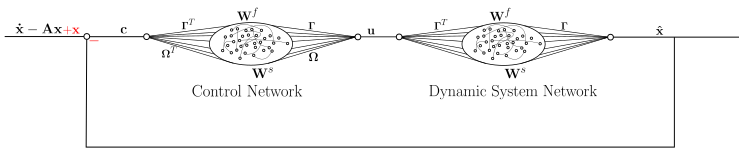
\includegraphics[width=\textwidth]{svg-inkscape/schematic_controller_network_feedback_2_nets.pdf}
		\caption{Add extra loop to introduce feedback into the control network.}
		\label{fig:schematic_feedback_control_2_nets}
	\end{subfigure}
	\vfill{1cm}
	\begin{subfigure}{\textwidth}
		\centering
		\includegraphics[width=\textwidth]{../../plots/everything/feedback_2_nets.pdf}
		\caption{Comparison of control for our model problem with the controlling and simulating network with and without feedback. Both runs used networks 50 neurons with identical parameters. Plots for $x_1$ and $x_2$ separately.}
		\label{fig:feedback_control_2_nets_error}

	\end{subfigure}
	\caption{Schematic to the addition of feedback in the in the control network. Additions are highlighted in red }
\end{figure}

While this improves performance, as seen in \cref{fig:feedback_control_2_nets_error}, the network output is still unusable due to the error.\\
Thus, efficient tracking is only possible using the analytically calculated matrices $\bmu{W}^f$ and $\bmu{W}^s$ and therefore disqualifies this approach as we aim to use the learned matrices.\\ Additionally, it was not possible to find training rules that would allow the training of the matrices used in the control network, posing further problems to our goal of using learning rules for the entire scheme.\\

\subsection{Merging 2 networks}
Unfortunately, the use off feedback did not help to achieve acceptable results. It is therefore necessary to make a trade-off between biologic plausibility and control scheme performance.\\
The alternative option being a combined network, incorporating both control and simulation at the same time.\\
As highlighted before, the governing force behind the control was not the network but rather only the definition of $\bmu{c}$. The network itself is primarily based around producing the necessary spikes and rates to return the corresponding control input $\bmu{u}$.
Therefore we construct a single network that handles both the control as well as the dynamic system itself. We define $\bmu{c}$ as
\begin{equation}
	\bmu{c} =  \bmu{\dot{x}}-\bmu{Ax}
\end{equation}
as before in the control network. In the current state, no control matrix is incorporated in the network which means that the network assumes $\bmu{B} = \bmu{I}$ which will be addressed later.\\

\subsubsection{Working as a open loop controller}
To begin we set a sine wave as our target. As can be seen in \cref{fig:all_open_sine_base}, the aforementioned control using $\bmu{c}$ appears to deliver good results using the optimal weights. Both state trajectories almost perfectly overlap the target. As seen before, similar to \cref{ssec:combining-2-network}, dynamics quickly diverge due to the imperfections in the learned matrices making it impossible for the open loop to properly control the system, leading to an almost complete loss of the target trajectory. Yet the output shows better tracking than the separate networks.
\begin{figure}
	\centering
	\includegraphics[width=\textwidth]{../../plots/everything/open_sine_base.pdf}
	\caption{Control results for the ideal and learned matrices $\bmu{W}^f$ and $\bmu{W}^s$ on a sine wave target. Top panel shows the $x_1$ state and bottom $x_2$. Matrices were trained for 1000 epochs using the previously studied optimal parameters.}
	\label{fig:all_open_sine_base}
\end{figure}
The error shown in \cref{fig:all_open_sine_base} is almost purely due to inaccuracies in $\bmu{W}^s$. If the control is rerun but instead the optimal $\bmu{W}^s$ are used with the learned $\bmu{W}^f$, greatly improved results can be obtained.\\
\begin{figure}
	\centering
	\includegraphics[width=\textwidth]{../../plots/everything/all_open_sine_base_ideal_Ws.pdf}
	\caption{Control results from \cref{fig:all_open_sine_base} but with only either $\bmu{W}^f$ or $\bmu{W}^s$ trained. Top panel shows the $x_1$ state and bottom $x_2$. Matrices were trained for 1000 epochs using the previously studied optimal parameters.}
	\label{fig:all_open_sine_base_ideal_Ws}
\end{figure}
In \cref{fig:all_open_sine_base_ideal_Ws} the results show that if the ideal $\bmu{W}^s$ is used, control accuracy is greatly improved. Small error still accumulate over time. These are from the remaining error in $\bmu{W}^f$ that is caused by small errors from training but also because $\bmu{W}^f$ adapts to the potential errors in $\bmu{W}^s$ during training. The opposite configuration yields even worse results, proving the principal error contribution stems from $\bmu{W}^s$.\\
As before, the main problem is that due to the open loop design very precise system information is necessary. With training, only a perturbed system $\bmu{A}' = \bmu{A} + \bmu{\varepsilon}$ of the system matrix is learned. Without state feedback, control over $\bmu{A}'$ produces different dynamics which cannot be compensated without state feedback.\\
This limits the applicability of any learned matrices.
\subsubsection{Adding Feedback}
In order to build a more robust controller, we add feedback to the control scheme as done before.\\
Although this can be done identically by adding the error term directly onto c, we can change the formulation here due to only one network being present.
While we still send add the target trajectory to $\bmu{c}$ we can move the feedback loop directly into the network. The network output is calculated by by $\bmu{\hat{x}} = \bmu{\Gamma r}$. Ignoring the subtraction, this value is then fed back into the network using the same weights using $\bmu{\Gamma}^T\bmu{c}$. It is therefore the same as keeping adding another matrix
\begin{equation}
\bmu{W}^e = -\bmu{\Gamma}^T\bmu{\Gamma}
\end{equation}
to the network dynamics. The negative sign is the subtraction we ignored earlier. The adjusted network dynamics are illustrated in \cref{fig:schematic_feedback_control}.
\begin{figure}
	\centering
	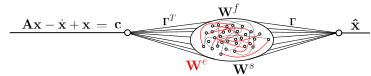
\includegraphics[width=\textwidth]{svg-inkscape/schematic_closed_loop_controller.pdf}
	\caption{Add extra loop to introduce feedback into our control scheme. The outside loop can be integrated into the network similarly to $\bmu{W}^s$.}
	\label{fig:schematic_feedback_control}
\end{figure}
To measure its effectiveness, we run the simulation with the added matrix. In \cref{fig:all_closed_feedback_extra_loop} we can clearly see the network performance is greatly improved. Both trajectories follow their target almost perfectly.\\
\begin{figure}
	\centering
	\includegraphics[width=\textwidth]{../../plots/everything/all_closed_sine_base.pdf}
	\caption{Control results from \cref{fig:all_open_sine_base} but with the added feedback loop seen in \cref{fig:schematic_feedback_control}.}
	\label{fig:all_closed_feedback_extra_loop}
\end{figure}


\subsubsection{Learning the new feedback loop}
Instead of introducing another matrix that is multiplied by the with the neuron firing rates, we can adjust the definition of $\bmu{W}^s$ to
\begin{equation}\label{eq:feedback_in_Ws}
\bmu{W}^s = \bmu{\Gamma}^T\left(\bmu{A} + (\lambda_d-1)\bmu{I} \right)\bmu{\Gamma}.
\end{equation}
This matrix can further be learned by the previous training algorithm by subtracting the identity matrix from $\bmu{A}$ before training.\\
We check if the learning of $\bmu{A-I}$ gives similar to results  with the extra loop in \cref{fig:all_closed_feedback_extra_loop}. We retrain our model problem using the identical parameter set as before with the identity matrix subtracted.\\
To measure whether the training was able to reproduce the subtraction we calculate the inner matrix of \cref{eq:feedback_in_Ws} using regression.
\begin{equation}
	\bmu{M^*} = \min_{\bmu{M}} \| \bmu{\Gamma}^T\left(\bmu{M}+\lambda_d\bmu{I}\right)\bmu{\Gamma} - \bmu{W}^s\|_2^2
\end{equation}
It shows that in this test case the training was able to resolve the subtraction with relative errors between matrix entries being less than 8\%.
In \cref{fig:all_closed_loop_learned} the result of training can be compared to the addition of the extra matrix after training. The final results is sufficiently accurate for almost perfect results. The target is tracked with almost identical performance as in \cref{fig:all_closed_feedback_extra_loop}
\begin{figure}
	\centering
	\includegraphics[width=\textwidth]{../../plots/everything/all_closed_loop_learned.pdf}
	\caption{Control results from \cref{fig:all_closed_feedback_extra_loop} but with the added feedback loop learned and integrated into the network directly.}
	\label{fig:all_closed_loop_learned}
\end{figure}

\subsubsection{Limitations on $\bmu{B}$}
All previous results are build on the implicit assumption of $\bmu{B} = \bmu{I}$. Although the results are acceptable, this assumption is prohibitively restrictive.\\
The easiest way to circumvent this restriction would be to have use the pseudo-inverse  $\bmu{B}^+$. If $\bmu{B}^+$ is available, the computations of network input can be simplified directly to
\begin{equation}\label{eq:feedback_with_B}
	\bmu{c} = \bmu{Bu}= \bmu{BB}^+\left(\bmu{\dot{x}- Ax}\right)
\end{equation}
if $\bmu{c} = \bmu{Bu}$ is substituted in the derivation of \cref{sec:simulation} and $\bmu{u} = \bmu{B}^+\left(\bmu{\dot{x} - Ax}\right)$,
ignoring the previously added feedback. But $\bmu{B}^+$ is often unavailable, moreover, biologically it is unrealistic to assume that the brain does matrix inversion. Instead, we restrict ourselves to matrices $\bmu{B}$ such that
\begin{equation}
	\bmu{BB}^+ = \bmu{BB}^T,
\end{equation}
which can be transformed to
\begin{equation}
\begin{aligned}
	\bmu{BB}^T &= \bmu{BB}^+\\
			  &= \bmu{B}\left(\bmu{B}^T\bmu{B}\right)^{-1}\bmu{B}^T\\
			  &\longrightarrow \bmu{B}^T\bmu{B} = \bmu{I}
\end{aligned}
\end{equation}
the condition that the Gram matrix of $\bmu{B}$ is the identity or the columns of $\bmu{B}$ form an orthonormal basis. The pseudo-inverse in \cref{eq:feedback_with_B} can then be replaced by $\bmu{B}^T$.\\

While this again is a strong limitation, it does increase the applicability of the network. To illustrate the this rerun the previous simulation with $\bmu{B} = [0,1]^T$ in \cref{fig:all_closed_1_net_with_b}
\begin{figure}
	\centering
	\includegraphics[width=\textwidth]{../../plots/everything/1_net_feedback_with_B.pdf}
	\caption{Control results from \cref{fig:all_closed_feedback_extra_loop} with the input matrix $\bmu{B} =[0,1]^T$.}
	\label{fig:all_closed_1_net_with_b}
\end{figure}
Unfortunately, the addition of $\bmu{B}$ ruins the network performance with the trained matrices. Again, this is mainly caused by inaccuracies in $\bmu{W}^s$, as the network shows perfect results in \cref{fig:all_closed_1_net_with_b} when both $\bmu{W}^s$ and $\bmu{W}^f$(\cref{fig:all_closed_1_net_with_b}) or just $\bmu{W}^s$(not shown) is computed analytically.\\
The main reason the network performs subpar is the addition of $\bmu{BB}^T$ towards the error signal before. As can be seen from \cref{fig:all_closed_1_net_with_b}, the error is primarily concentrated in the $x_1$ state which is not directly accessible by neither the error signal nor the network input $\bmu{c}$ due to
\begin{equation}
	\bmu{BB}^T = \begin{bmatrix}
	0&0\\
	0&1\\
	\end{bmatrix}
\end{equation}
removing any potential control over $x_1$, causing small inaccuracies to let the network diverge over time.\\

\subsection{Limitations}
The main limitation of the approaches presented here is the learning accuracy of $\bmu{W}^s$.
Both presented approaches deliver good results with analytically computed matrix weights. Either of them is useable to control a system if $\bmu{W}^s$ calculated analytically.\\
Only if either $\bmu{B}$ or the learning is neglected, both approaches can perform accurately. Ignoring $\bmu{B}$ hugely limits the applicability of the whole network in spite of the accurate results. To the above mentioned limitations all the limitations of previous sections also apply. This concerns especially the application to bigger systems, random initialization of weights before training or the choice of $\bmu{\Gamma}$.\\
The addition of the error signal is necessary in order to balance the network noise. Due to lack of feedback, it is impossible to be accounted for. Therefore inherent noise in the network is completely unchecked.
Noise can alternatively be mitigated by scaling $\bmu{\Gamma}$ and the subsequent threshold to small scales. In this case, the amount to spikes to represent the same signal will be increased, reducing the relative importance of spikes caused by noise. By doing this, the network is basically converted into a classic rate network.\\
